\chapter{Asking Politicians How They Actually Got Rich!}

This chapter is best read as a field lecture rather than as a studio interview. We begin outside the Capitol in refusal, hurry, and partial access; only gradually does the scene yield usable doctrine. From there the lecture moves through four distinct mechanisms: first-asset finance, reputation built by service, long-horizon entrepreneurial accumulation, and the arithmetic of debt, information, and votes inside Washington. No validated board equations survive for this lecture, so the mathematics below is intentionally light and schematic. Its purpose is not to over-formalize the interview, but to stabilize the mechanisms that the speakers themselves keep returning to.

\section{Access Friction at the Capitol}

The opening rhythm matters. The host does not begin with a settled argument. He begins with a question that is simple enough to be almost naive: when did you make your first million? In Washington that question does not land cleanly. People are moving between meetings, declining to speak, deflecting, or revealing only after a moment that they are not merely passersby but members of Congress. The lecture therefore opens by teaching a condition of inquiry: before we can extract a mechanism, we have to get a subject to stop.

We can summarize that access structure by a small schematic:
\begin{equation}
\text{cold approach}\to \text{refusal / motion}\to \text{brief stop}\to \text{usable doctrine}.
\end{equation}
This is not an incidental preface. It tells us how the material is to be read. Politics here is not transparent exposition. It is a guarded environment in which a claim must be caught in transit.

\begin{figure}[h]
\centering
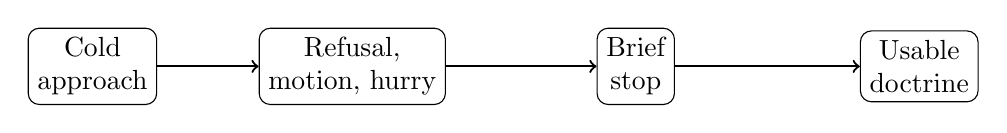
\begin{tikzpicture}
\node[draw, rounded corners, align=center] (a) at (0,0) {Cold\\ approach};
\node[draw, rounded corners, align=center] (b) at (3.3,0) {Refusal,\\ motion, hurry};
\node[draw, rounded corners, align=center] (c) at (6.9,0) {Brief\\ stop};
\node[draw, rounded corners, align=center] (d) at (10.5,0) {Usable\\ doctrine};
\draw[->, thick] (a) -- (b);
\draw[->, thick] (b) -- (c);
\draw[->, thick] (c) -- (d);
\end{tikzpicture}
\caption{The lecture's opening method: knowledge is extracted in motion, not presented in a settled classroom format.}
\end{figure}

After this pressure the mission is stated explicitly. The host is in Washington, D.C.\ for the first time, and he is looking not merely for personal stories but for the connection between wealth, politics, and what government actors may know that others do not. Once that frame is in place, the first real mechanism arrives.

\section{Mike Collins: One Truck, One Bank, One Scalable Base}

Mike Collins gives the lecture its first clean business spine. He says that he started his first business at age $23$, that he was in trucking, that he began with one truck, and that the operation now runs over one hundred a day. He adds a brokerage company and gives a revenue band for a strong year. The transcript does not support an audited balance sheet, but it does support a scale ladder:
\begin{align}
N_{\text{trucks}} &: 1 \to 100+,\\
R_{\max} &\in [20,50]\ \text{million USD}.
\end{align}

That pair of facts is enough to orient the whole segment. The visible size is large, but the lecture does not begin with scale; it begins with the first productive asset.

\subsection{Question \& Answer}

\paragraph{Question.} How does someone buy the first productive asset without inherited capital?

\paragraph{Answer.} Collins answers in the oldest possible entrepreneurial language: he went to a small community bank, and that bank knew its customer. We should not invent loan terms, collateral ratios, or formal underwriting details. But we can write the mechanism in a cautious standard form:
\begin{equation}
\text{local bank knowledge}\to \text{credit}\to \text{first truck}\to \text{operating revenue}\to \text{scale}.
\end{equation}
The point is not that community banking is romantic. The point is that local information changes the lending situation. A bank that knows the person, the family, and the community does not face the same kind of abstract uncertainty as a distant institution. The first truck is therefore not a miracle and not a theorem; it is the first place where reputation, locality, and productive capacity meet.

\begin{figure}[h]
\centering
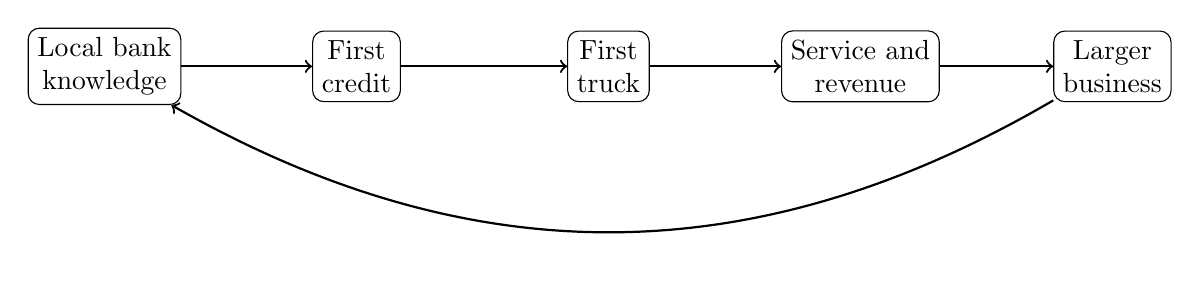
\begin{tikzpicture}
\node[draw, rounded corners, align=center] (a) at (0,0) {Local bank\\ knowledge};
\node[draw, rounded corners, align=center] (b) at (3.2,0) {First\\ credit};
\node[draw, rounded corners, align=center] (c) at (6.4,0) {First\\ truck};
\node[draw, rounded corners, align=center] (d) at (9.6,0) {Service and\\ revenue};
\node[draw, rounded corners, align=center] (e) at (12.8,0) {Larger\\ business};
\draw[->, thick] (a) -- (b);
\draw[->, thick] (b) -- (c);
\draw[->, thick] (c) -- (d);
\draw[->, thick] (d) -- (e);
\draw[->, thick, bend left=30] (e) to (a);
\end{tikzpicture}
\caption{A cautious transcript-derived reconstruction of Collins's first-asset mechanism. The return arrow indicates that successful execution feeds back into future finance and credibility.}
\end{figure}

\section{From Local Credit to Service and Incentive}

Once Collins has given the first-truck story, the lecture widens. He shifts from a single financing episode to a thesis about free markets, small business, risk, and the damage done when local credit is lost. Here we have to keep the layers separate. The claims about government, markets, and political parties remain his claims. The mechanism, however, is commercially intelligible and can be stated without overreaching.

The commercial core of his differentiation is not bigness. It is service. The firm is not necessarily the biggest, but it does what it says it will do. When something goes wrong, it compensates, re-routes, repairs, and continues. That suggests a simple update rule for trust:
\begin{equation}
T_{t+1}=T_t+\Delta T_t,\qquad \Delta T_t>0
\end{equation}
whenever a commitment is fulfilled, or a disruption is competently repaired.

We can make the recurrence explicit. If we let $\delta_i$ denote the trust increment generated by the $i$th fulfilled or repaired commitment, then
\begin{align}
T_1 &= T_0+\delta_1,\\
T_2 &= T_1+\delta_2 = T_0+\delta_1+\delta_2,\\
T_n &= T_0+\sum_{i=1}^n \delta_i.
\end{align}
This is the cleanest mathematical example in the Collins material. One does not need to be the largest operator in the field. One needs repeated positive increments in trust stock. That is why customers call back, and it is also why Collins draws an analogy to politics itself: if representatives simply did their job, people would reward that too.

The lecture also uses Collins to state an incentive claim. Small business requires retained upside. A free market, in his language, is valuable because it preserves the incentive to start from the ground up, take a risk, and work one's way up. We should note the claim, but we should not pretend the lecture gives a full model of the market. The stable note is simply this: entrepreneurial effort here is narrated as effort under conditions where upside still belongs, at least in part, to the builder.

\subsection{Question \& Answer}

\paragraph{Question.} Is hard work by itself enough?

\paragraph{Answer.} Not in the form this lecture gives us. Collins never abandons hard work, but he does refine it. Work without reliability is just exertion. Work that becomes observable service enters the reputation recurrence above and therefore changes the future call pattern. In the lecture's own rhythm, effort becomes commercially visible only when it is tied to delivery.

\section{Gregory Meeks: Education, Reading, and the First Change in Trajectory}

After a host recap the lecture resets. We are back outside the Capitol, back in motion, and then the next strong stop takes a different path. Gregory Meeks does not begin with a first truck or a first company. He begins with public housing, poverty, and responsibility. The frame shifts from wealth accumulation narrowly understood to family trajectory and civic responsibility.

The first actionable step is not mysterious. Meeks says that for him the first thing was education; then family, then reading, then learning what was happening around him, and then asking how he could make a difference. The sequence is structural, and it is worth preserving in exactly that form:
\begin{equation}
\text{public housing}\to
\text{education}\to
\text{reading}\to
\text{environment awareness}\to
\text{contribution}\to
\text{office}.
\end{equation}
This is not a numerical derivation. It is a state progression. It matters because the lecture is refusing a false simplification. Not every route to institutional power runs first through business scale. Some routes run through literacy, awareness, contribution, and public action.

There is also a valuable scale marker embedded in the exchange. Meeks notes that there are only ``about five hundred or so'' people in the House of Representatives. We should leave this approximate, as the lecture does:
\begin{equation}
N_{\text{House}} \approx 500.
\end{equation}
The point is not numerical civics precision; the point is rarity. The office is rare, and the trajectory into it is therefore a trajectory into a very small institutional set.

Faith enters this section in a different way than it did with Collins. Meeks does not use it primarily to explain unexpected business openings. He uses it to describe decision, moral orientation, and the attempt to do what is right, humane, and godly. Then the lecture raises one of its most important tensions: if politics is nasty, why enter it at all? Meeks answers that politics is how things are changed, and that the civil-rights movement created the right for him to be there. In this interview, office is not presented as a monetization opportunity. It is presented as an inherited obligation.

\subsection{Question \& Answer}

\paragraph{Question.} What is the first actionable step in changing a family's trajectory?

\paragraph{Answer.} In this lecture the answer is not abstract inspiration. It is ordered practice: education first, then reading, then awareness, then contribution. The sequence matters because it turns a social condition into a path rather than into a slogan.

\section{The Montana Route: Startup, Yahoo, and the Decade Game}

The next major interview returns to classical entrepreneurship, but now with a longer arc. The representative from Montana gives a chain that runs from poverty to college to NYU research, then from teaching to a startup, from the startup to a pooling-of-interests merger with Yahoo, and from there to angel financing and early-stage venture support. Again, we should not invent cap-table details. But we can preserve the business logic: the career compounds by repeated construction, not by one theatrical leap.

This is the right place to write the lecture's long-horizon recurrence:
\begin{equation}
B_{t+1}=B_t+\Delta B_t,\qquad \Delta B_t>0
\end{equation}
under continued execution.

Unfolding the recurrence over many periods gives
\begin{equation}
B_n = B_0+\sum_{i=0}^{n-1}\Delta B_i.
\end{equation}
That is the mathematics of ``turning the crank.'' Each increment may be modest, but the sum across years is not. The speaker's criticism of the phrase ``overnight success'' is therefore quite sharp: what looks sudden at the end is usually a cumulative integral of ordinary increments.

The lecture underlines the point by adding a work-intensity band from the speaker's early tech years:
\begin{equation}
h_{\text{work}} \approx 20\ \text{hours/day},\qquad s_{\text{sleep}} \approx 4\ \text{hours/night}.
\end{equation}
We should preserve these as self-reported anchors, not as prescriptions. Their function in the lecture is to reject the myth of effortless ascent.

\subsection{Question \& Answer}

\paragraph{Question.} Why does ``overnight success'' still require decades?

\paragraph{Answer.} Because the visible outcome is a terminal snapshot, while the real process is cumulative. In the lecture's own language, one keeps turning the crank, keeps the ball moving down the field, and only later looks back at what has been built. Formally, the end state is a sum of increments, not a single jump.

This section also contains a crucial political pivot. After narrating his own path, the speaker turns to the America that made such a path possible and argues that the opportunity is being squandered. Homeownership, family formation, and small-business entry appear here as threatened goods. The bridge to fiscal politics is now complete.

\section{Byron Donalds: Debt Arithmetic and Insider Asymmetry}

Byron Donalds gives the lecture its cleanest public-finance spine. His route into politics begins in finance, in research done during the 2008 crisis, and in the realization that the institutional story mattered. From there the lecture moves into arithmetic that is loose in form but precise in direction.

The first claim is that one cannot borrow forever. The second is that more borrowing raises the cost burden. The third is that increased debt destroys purchasing power, with poor people and seniors on fixed incomes taking the first blow. A cautious standard form of the claim is
\begin{equation}
D'(t)>0 \Rightarrow \text{cost burden rises} \Rightarrow P_{\text{pp}}(t)\downarrow.
\end{equation}
Here $D(t)$ is the national debt path and $P_{\text{pp}}(t)$ is the purchasing power of ordinary Americans. This is not a calibrated macro model. It is a compact rendering of the mechanism Donalds wants the listener to notice.

\subsection{Question \& Answer}

\paragraph{Question.} If the government cannot stop borrowing immediately, what does it mean to slow the trajectory first?

\paragraph{Answer.} The distinction is between the level of debt and the slope of the debt path. One can still have a rising debt stock while reducing the speed at which it rises:
\begin{equation}
D'_{\text{slowed}}(t)<D'_{\text{current}}(t),
\end{equation}
even if both derivatives remain positive at first.

This matters over time. If the current path and the slowed path start together, then after a horizon $T$ their gap is
\begin{equation}
D_{\text{current}}(T)-D_{\text{slowed}}(T)
=
\int_0^T \bigl(D'_{\text{current}}(t)-D'_{\text{slowed}}(t)\bigr)\,dt.
\end{equation}
If the integrand stays positive, the gap widens with time. That is the mathematical content of ``slow the trajectory first.'' It does not yet mean debt has been paid down. It means the path has become less steep, which is the lecture's immediate target before any longer-horizon paydown plan.

\begin{figure}[h]
\centering
\begin{tikzpicture}
\draw[->] (0,0) -- (6.5,0) node[right] {$t$};
\draw[->] (0,0) -- (0,4.5) node[above] {$D(t)$};
\draw[thick] (0.4,0.5) .. controls (2,1.0) and (4,2.0) .. (6,4.0);
\draw[thick] (0.4,0.5) .. controls (2,0.9) and (4,1.6) .. (6,2.8);
\node at (5.0,3.8) {$D_{\text{current}}$};
\node at (4.8,2.5) {$D_{\text{slowed}}$};
\end{tikzpicture}
\caption{A transcript-derived debt picture. Both paths may rise initially; the point is that the slowed path has a smaller slope before any later attempt at paydown.}
\end{figure}

The same section gives an ethics argument about congressional trading. Donalds says directly that members have information other people do not. The clean notation is
\begin{equation}
I_{\text{member}} > I_{\text{public}}.
\end{equation}
From this he infers not market efficiency but ethics: if members trade directly while sitting inside that asymmetry, the practice is compromised. He therefore delegates trading to a firm and says openly that he thinks direct member trading is unethical.

The lecture then presses further. If office can be turned into a private enrichment machine, politics stops being about the people who sent the representative. That is why Donalds says that if one does the job correctly, one loses money on the deal. Again, we should preserve the moral claim without turning it into an accounting identity.

\section{Fear, Votes, and the Person Behind the Office}

The Donalds material does not stop with debt. It moves next into institutional power. The striking claim is that most members are afraid: afraid of criticism, afraid of the difficult right decision, afraid of the immediate cost of boldness. The lecture then asks who really holds power in Washington. The answer names the president and legislative leaders, but then shifts to a more operational standard: counted votes.

That mechanism can be written in the simplest possible way:
\begin{equation}
V\ge V_{\text{majority}} \Rightarrow \text{floor action},\qquad
V<V_{\text{majority}} \Rightarrow \text{stasis}.
\end{equation}
The important thing is not the symbol. The important thing is the explanatory shift. Real power is not merely title; it is coalition arithmetic. A disciplined cluster of members willing to stand firm can change outcomes because, in the end, everyone is counting votes.

This logic also explains why the speaker defends term limits. If power can corrupt and if the institution rewards long occupancy, then periodically going home becomes part of the safeguard. The lecture does not develop a formal theorem of institutional decay, but the direction is clear.

From here the interview moves from public mechanism back to personal formation. Donalds recalls being advised at age $29$ to get to where he wanted to get to by $40$, because that is where money and mark really begin to compound:
\begin{equation}
a_{\text{advice}}=29,\qquad a_{\text{target}}=40.
\end{equation}
This is not a deterministic law. It is a life-course heuristic. The early years are for grinding, learning how to work, and learning how to work with others. The later years are where compounding becomes visible.

Then comes the sharper threshold. Donalds describes arrests at ages $18$ and $20$, and then says that at $20$ he made a decision: he was not going to be in that position again. The mathematically useful way to preserve this is as a state change rather than as a continuous drift:
\begin{equation}
S_{20^-}\xrightarrow{\text{decision at }20} S_{20^+}.
\end{equation}
The lecture insists on the discreteness of this moment. The change is not described as statistical improvement. It is described as a threshold act of self-command.

Faith then stabilizes the path. He gives his life to Christ at $21$, later explains the Cracker Barrel conversion story, and frames subsequent life not as victimhood but as guidance, responsibility, and execution. The host asks whether the system is rigged. Donalds replies that people are missing the playbook. This answer should not be flattened into optimism. It is a rebuke to passivity: one must run the play.

\subsection{Question \& Answer}

\paragraph{Question.} What changes first: the system around us, or the decision we make in the mirror?

\paragraph{Answer.} This lecture answers in two stages. Public systems matter enormously; debt paths, information asymmetries, and vote thresholds are real. But the transition into agency begins with a personal threshold. One decides, then one works, then one compounds. The public and the private are not alternatives here. They are sequentially braided.

\section{Summary}

The lecture begins in motion and ends in structure. First we see how hard it is to get anyone in Washington to stop long enough to speak. Then we get the first-asset mechanism from Collins: local knowledge, first credit, first truck, scale. Next we get a second route from Meeks: education, reading, awareness, contribution, office. Then the Montana interview gives the recurrence of long-horizon building and punctures the myth of overnight success. Finally Donalds supplies the cleanest public arithmetic: debt trajectories, purchasing power, insider-information ethics, coalition voting, and the role of self-command in moving through the institution.

What remains after the chapter is not a single theory of wealth. It is a linked set of mechanisms. Productive assets matter. Local trust matters. Repeated service matters. Time matters. Public debt is not abstract if it reaches down into household purchasing power. Political office is not identical with power if votes are missing. And the person who enters such a system is still, at crucial moments, the person who must decide what sort of life to lead.